\documentclass{beamer}

\usepackage{graphicx}

\usecolortheme[named=blue]{structure}

\mode<presentation>
{
  \usetheme{Warsaw}
  \setbeamercovered{transparent}
  \setbeamertemplate{items}[ball]
  \setbeamertemplate{theorems}[numbered]
  \setbeamertemplate{footline}[frame number]
  
% custom colors
  \setbeamercolor{structure}{fg=red!90!black}
  
  \setbeamerfont{section number projected}{%
  	family=\rmfamily,series=\bfseries,size=\normalsize
  }
  \setbeamercolor{section number projected}{bg=red,fg=white}
  \setbeamercolor{frametitle in head}{fg=Brown,bg=Brown!20}
  
}

% \usecolortheme{spruce}

\usepackage{beamerthemesplit}
\usepackage{graphics}
\usepackage{graphicx}
\usepackage{hyperref}
\usepackage{color}
\usepackage{listings}
\usepackage[utf8]{inputenc}

\newcommand{\code}[1]{\texttt{\small{#1}}}
\hypersetup{%
  colorlinks=true,
  urlcolor=red,
  linkcolor=red,
  pdfborderstyle={/S/U/W 1}
}

\definecolor{javared}{rgb}{0.6,0,0} % for strings
\definecolor{javagreen}{rgb}{0.25,0.5,0.35} % comments
\definecolor{javapurple}{rgb}{0.5,0,0.35} % keywords
\definecolor{javadocblue}{rgb}{0.25,0.35,0.75} % javadoc

\lstdefinelanguage{scala}{
  morekeywords={abstract,case,catch,class,def,%
    do,else,extends,false,final,finally,%
    for,if,implicit,import,match,mixin,%
    new,null,object,override,package,%
    private,protected,requires,return,sealed,%
    super,this,throw,trait,true,try,%
    type,const,var,while,with,yield},
  otherkeywords={=>,<-,<\%,<:,>:,\#,@,>,<},
  sensitive=true,
  morecomment=[l]{//},
  morecomment=[n]{/*}{*/},
  morestring=[b]",
  morestring=[b]',
  morestring=[b]"""
}
\lstset{
%   frame=tb,
  language=Scala,
  aboveskip=3mm,
  belowskip=3mm,
  columns=flexible,
  basicstyle=\ttfamily\small,
  keywordstyle=\color{javapurple}\bfseries,
  stringstyle=\color{javared},
  commentstyle=\color{javagreen},
  morecomment=[s][\color{javadocblue}]{/**}{*/},
  numbers=none,
  numberstyle=\tiny\color{black},
  stepnumber=2,
  numbersep=10pt,
  showspaces=false,
  showstringspaces=false,
  tabsize=4
}

\newcommand{\screenshot}[1]{\centerline{%
    \includegraphics[height=7.8cm,transparent]{#1}}}  % 7.8in

\title
  [Enseñando progamación]
  {Enseñando programación para el desarrollo profesional}
\author[Passerini]{%
  Nicolás Passerini\inst{1} \and
  Fernando Dodino\inst{1,2,3} \\
  Javier Fernandes\inst{1} \and
  Pablo Tesone\inst{4} \and
  Carlos Lombardi\inst{1}
}  

\institute{
  \inst{1}Universidad Nacional de Quilmes \\
  \inst{2}Universidad Nacional de San Martin \\
  \inst{3}Universidad Nacional del Oeste \\
  \inst{4}Institut National de Recherche en Informatique et en Automatique.
}

\date[FLISoL UNQ 2017]{\small Festival Latinoamericano de Instalación de Software Libre\\
Universidad Nacional de Quilmes\\
22/4/2017}
\subject{Computational Sciences}

%\logo{\includegraphics[height=1.0cm]{fsu_logo.pdf}}

\begin{document}
  \frame
  {
    \titlepage
  }

  \frame
  {
    \frametitle{Agenda}
    \tableofcontents
  }

\section{Introduccion}
\defverbatim[colored]\helloWorldJava{
\begin{lstlisting}[language=Java]
		package examples;
		
		public class HelloWorld {
			public static void main(String[] args) {
				System.out.println("Hello World");
			}
		}
\end{lstlisting}
}

\frame{
	\frametitle{Contexto}
	\begin{itemize}
	    \item Nos interesa la enseñanza de \textbf{programación con objetos}
	    \medskip
	    \item Principalmente en tecnicaturas e ingenierías
	    \begin{itemize}
    		\item es decir: futuros desarrolladores de software
	    \end{itemize}
	    \medskip
	    \item Fundamentalmente universitarios
	    \begin{itemize}
	    	\item Pero también estamos trabajando con secundarios
	    \end{itemize}
	\end{itemize}
}

\frame{
	\frametitle{Problema}
	\begin{itemize}
		\item Bajos niveles de aprobación
		\pause
		\item Suelen propagarse malas prácticas de programación
		\item Dificultades en la comprensión de los conceptos básicos
		\item Baja calidad del código producido
	\end{itemize}
	\pause
	\bigskip
	¿Por qué pasa eso?
	\begin{itemize}
		\item Capacidad de abstracción insuficiente
		\item Base matemática débil
	\end{itemize}
	\pause
	\bigskip
	Es nuestra responsabilidad cubrir esas falencias.
}

\frame{
	\frametitle{¿Por qué es difícil aprender OOP?}	
	\begin{itemize}
    \item Enfoque en un lenguaje particular
    \item Demasiados conceptos
    \medskip
    \helloWorldJava
    \pause
    \item \textbf{Entornos de desarrollo} limitados o inadecuados
    \item Aprender a programar exige \textbf{aprender a abstraer}
	\end{itemize}
}

\frame<0>[noframenumbering]{
	\frametitle{Introducción}
	\framesubtitle{Antecedentes}
	
\includegraphics[width=9pt,
			 	height=9pt,natwidth=66pt,natheight=50pt]{images/ozono-icon.png}
	\textbf{Ozono} \hfill \texttt{\footnotesize
	\href{http://ozono.uqbar-project.org/}{http://ozono.uqbar-project.org/}}
	\begin{itemize}
		\item Basado en Smalltalk
		\item \textbf{Recorrido incremental}
		\\\hspace{2em} Metamodelo simplificado: sin clases ni herencia
		\\\hspace{2em} Foco en objeto - mensaje - referencia - polimorfismo
		\item Herramientas de visualización de código
		\\\hspace{2em} Diagramas de objetos / clases
	\end{itemize}
	
	\pause\bigskip
	
\includegraphics[width=9pt,
			 	height=9pt,natwidth=313pt,natheight=365pt]{images/gobstones-icon.png}
	\textbf{Gobstones} \hfill \texttt{\footnotesize
	\href{http://www.gobstones.org/}{http://www.gobstones.org/}}
	\begin{itemize}
		\item Cuidadosa selección de los elementos sintácticos
		\item Elimina la necesidad de entrada-salida
		\item Separación entre elementos con efecto y elementos puros
	\end{itemize}
}

\frame{
	\frametitle{Propuesta pedagógica}
	\framesubtitle{Objetivos}
	\begin{itemize}
		\item \textbf{Inclusión}
		\\ Diseñar la currícula a partir de las características de los estudiantes.
		\medskip
		\item \textbf{Calidad}
		\\ A la vez que incrementar la calidad
		\medskip
		\item \textbf{Aplicabilidad}
		\\ Asegurando que los saberes impartidos sean aplicables en el ámbito profesional actual y futuro
		\medskip
		\item \textbf{Perspectiva futura}
		\\ Y liderando el desarrollo y la incorporación de nuevas ideas y tecnologías
	\end{itemize}
}

\frame{
	\frametitle{Propuesta pedagógica}
	\framesubtitle{Pilares}
	\begin{itemize}
		\item Temario y recorrido
		\item Seguimiento
		\item Deducción, intuición, autonomía
		\item Soporte de herramientas
	\end{itemize}
}

\frame{
	\frametitle{Introducción}
	\framesubtitle{¿Qué es Wollok?}
	\begin{itemize}
	 \item Lenguaje + muchas herramientas
	 \item Soporte para nuestro enfoque pedagógico
	 \item Cercanos a las herramientas profesionales \emph{mainstream}
	\end{itemize}
	
	\begin{center}
		\begin{figure}
			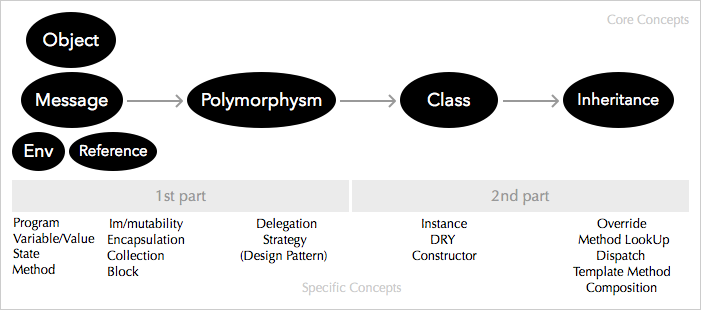
\includegraphics[height=0.5\textheight,natwidth=701,natheight=310]{images/wollok-learning-path.png}
		\end{figure}
	\end{center}
}

\frame{
	\frametitle{Introducción}
	\framesubtitle{¿Qué es Wollok? - Un entorno optimizado para la enseñanza}
	\begin{itemize}
		\item Sintaxis cuidada 
			\begin{itemize}
			  \item selección de keywords (ej: \code{const}, \code{method})
			  \item \code{return} obligatorio
			  \item énfasis en objetos y mensajes \footnote {¡Aunque no todo es objeto-mensaje!}
			\end{itemize}
		\item Combina \textit{object-based} con \textit{class-based programming}
		\item APIs minimalistas (ej: colecciones)
		\item \textit{Import system}
	\end{itemize}
}

\frame{
	\frametitle{Introducción}
	\framesubtitle{Cuidado: No perderle pisada la evolución de las herramientas industriales}
	\begin{itemize}
		\item Ambiente de objetos basado en archivos
		\item Framework de testing integrado
		\item Sintaxis concisa y "moderna"\\
		{\footnotesize Ej: lambdas, literales para colecciones, excepciones, constructores}
		\item Sistema de tipos \emph{pluggeable} (en proceso)
		\item Mixins
	\end{itemize}
}

%
% FEATURE AVANZADOS
%

\section{Características}
\frame{
	\frametitle{Características}	
	\begin{itemize}
    \item Reporte de errores adaptado e internacionalizado.
    \item Testeo automático integrado.
    \item ContentAssist, quick fixes, refactorings, formateo automático.
    \item Diagramas estáticos (y dinámicos en proceso).
    \item Versionado y trabajo en grupo (básico).
    \item Debugger (en proceso).
    \item Soporte para editores livianos (Sublime) y web (Mumuki, otros en proceso).
	\end{itemize}
}

\frame{
	\frametitle{Características}
	\framesubtitle{Tests}
	Tests
	\begin{center}
		\begin{figure}
			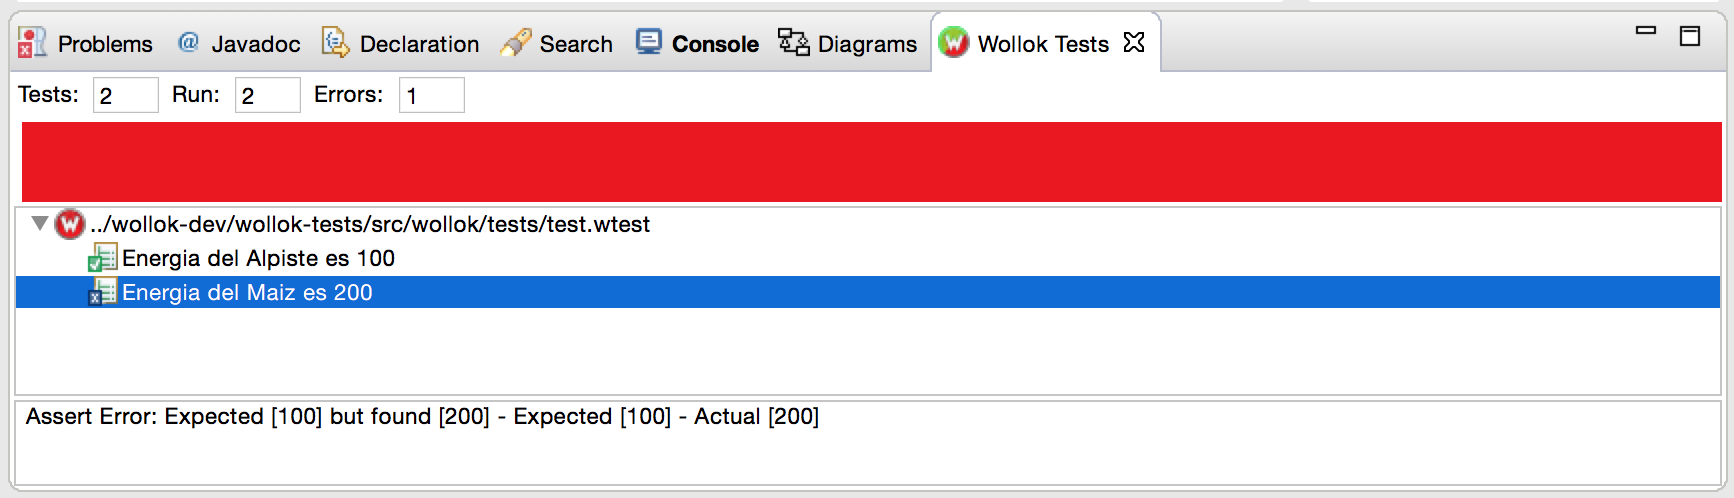
\includegraphics[width=1\textwidth,natwidth=1734,natheight=498]{images/tests.png}
		\end{figure}
	\end{center}
}

\frame{
	\frametitle{Sublime Support}
	\framesubtitle{Syntax Highlight}	
	\begin{center}
		\begin{figure}
			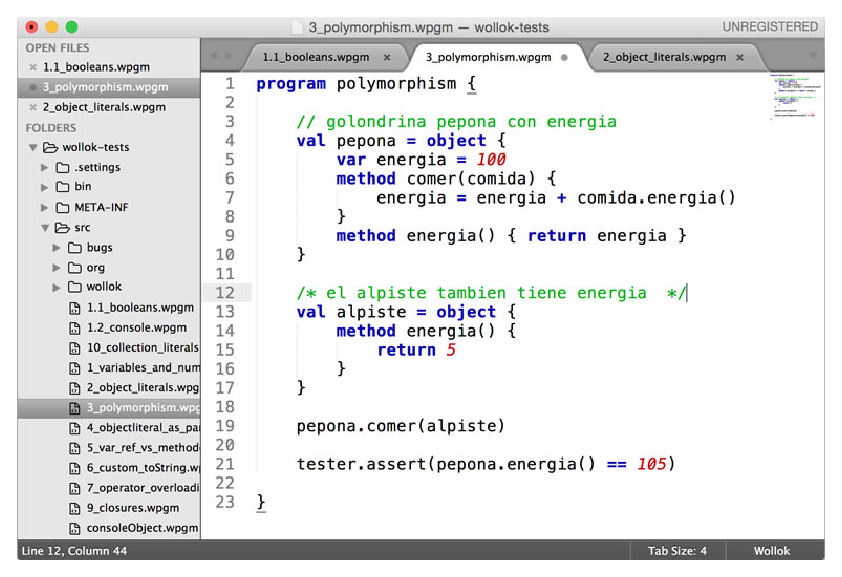
\includegraphics[height=0.8\textheight,natwidth=800,natheight=561]{images/wollok-wisit-sublime-syntax.eps}
		\end{figure}
	\end{center}
}

\frame{
	\frametitle{Sublime Support}
	\framesubtitle{Linter}
	\begin{center}
		\begin{figure}
			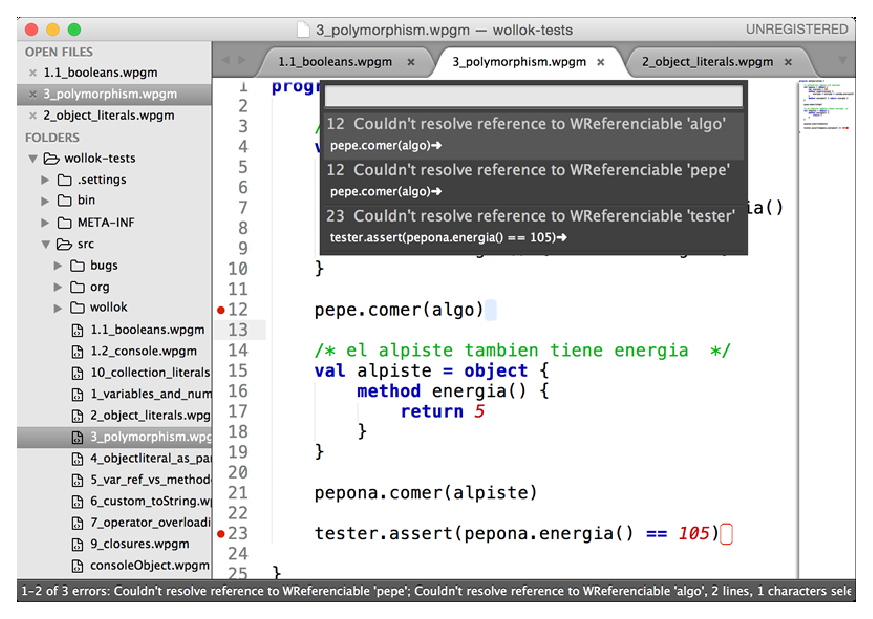
\includegraphics[height=0.8\textheight,natwidth=800,natheight=558]{images/wollok-wisit-sublime-linter.eps}
		\end{figure}
	\end{center}
}

\frame{
	\frametitle{Características}
	\framesubtitle{Debugger}
	Debugger
	\begin{itemize}
	    \item UI integrada a Eclipse Debug
	    \item Breakpoints: agregar, remover, deshabilitar, etc
	    \item Step, into, out 
	    \item Inspeccionar variables
	    \item Diagrama de Objetos
	\end{itemize}
}

\frame{
	\frametitle{Características}
	\framesubtitle{Soporte para Sublime}
	Soporte para Sublime
	\begin{itemize}
	    \item WDK
	    	\begin{itemize}
	    		\item No IDE
	    		\item $\sim70$MB (vs $\sim140$)
	    		\item Headless: wchecker, winterpreter, wtest
	    	\end{itemize}
	    \item Syntax highlight
	    \item Templates 
	    \item Linter
	\end{itemize}
}

%
% WOLLOK GAME
%

\section{Wollok Game}
\frame{
	\frametitle{Wollok Game}
	\begin{itemize}
		\item Herramienta complementaria al testeo unitario y consola interactiva.
		\item Mejorar la comprensión de conceptos.
		\item Visualización de comportamiento
		\item Motivación en el aprendizaje fomentando la participación.
	\end{itemize}
}

\frame{
	\frametitle{Wollok Game}
	\framesubtitle{FarmVille}
	\textbf{FarmVille} - Demo
	
	\begin{center}
		\begin{figure}
			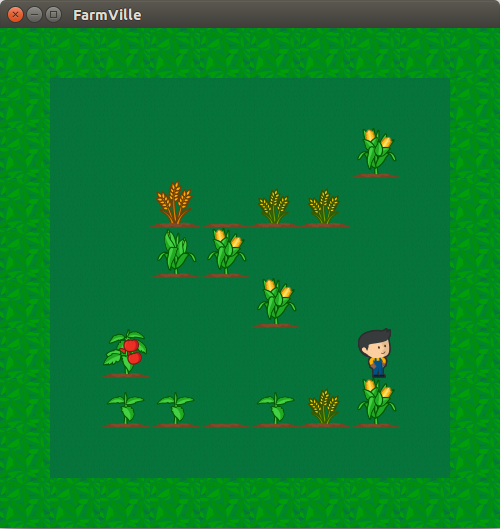
\includegraphics[width=0.4\textwidth,height=0.6\textheight,natwidth=500,natheight=529]{images/wollok-game-farmville.png}
		\end{figure}
	\end{center}
}

\frame{
	\frametitle{Wollok Game}
	\framesubtitle{Sokoban}
	\textbf{Sokoban} - Demo
	
	\begin{center}
		\begin{figure}
			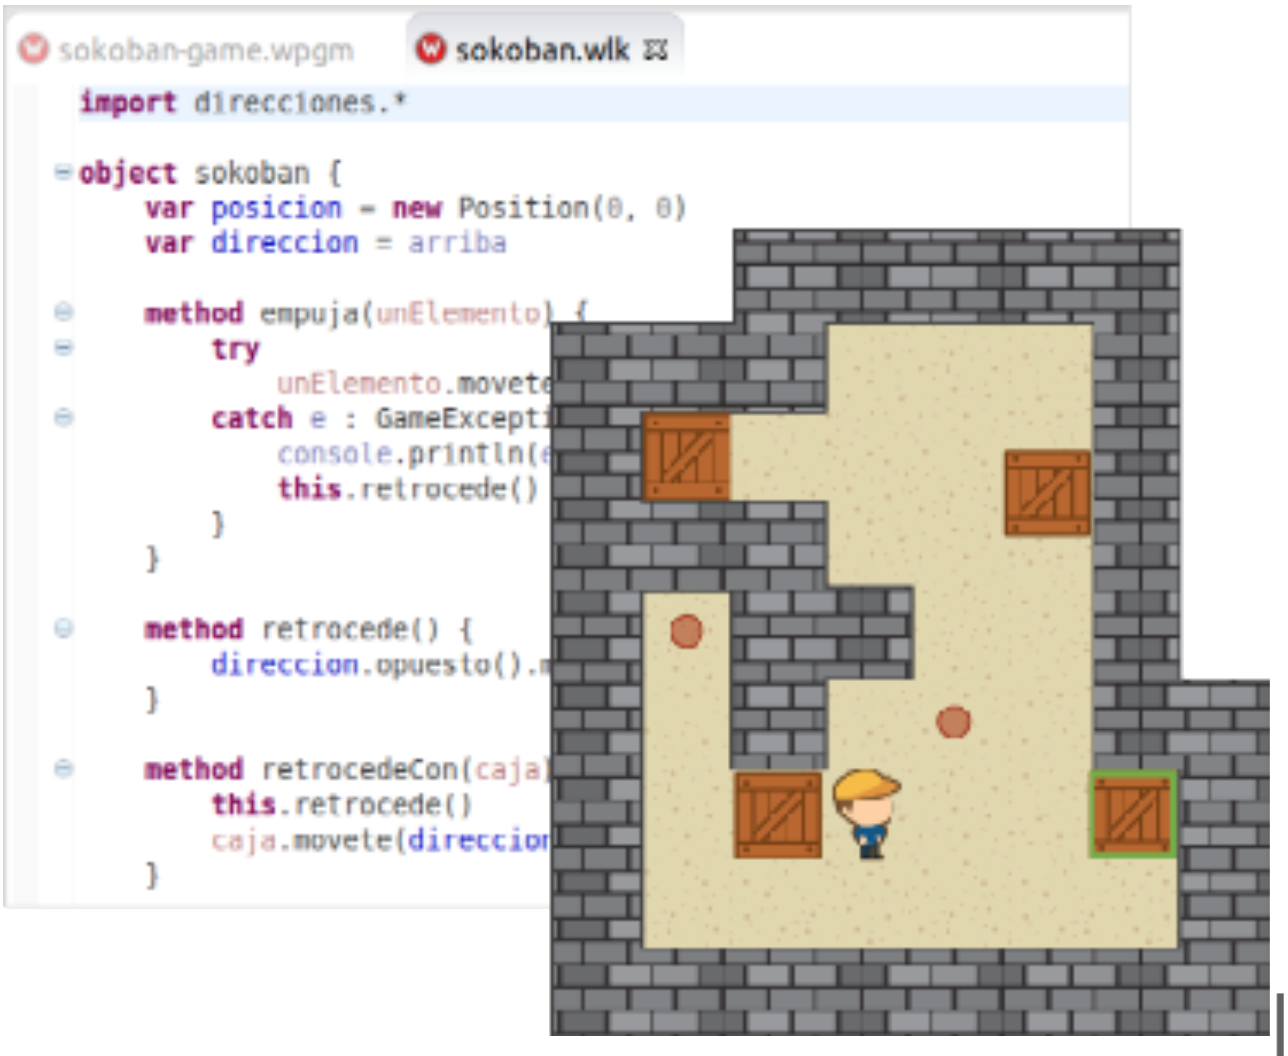
\includegraphics[width=0.4\textwidth,height=0.6\textheight,natwidth=258,natheight=289]{images/wollok-game-sokoban.png}
		\end{figure}
	\end{center}
}

\frame{
	\frametitle{Wollok Game}
	\framesubtitle{Futuro}
	Futuro
	\begin{itemize}
		\item + Tipos de \textbf{Juegos}
		\begin{itemize}
		  \item Survival
		  \item Por turnos
		\end{itemize}
		\item + Tipos de \textbf{Interacciones}
		\item Features Gráficos
		\begin{itemize}
		  \item Animaciones
		  \item Fondos infinitos
		  \item Distintos vistas (lateral, isométrica, etc)
		\end{itemize}
	\end{itemize}
}

\section{Experiencia en el Aula}
\frame{
	\frametitle{Experiencia en el Aula}
	Los alumnos se apropian intuitivamente de las herramientas
	\begin{itemize}
		\item Integración class-based / object-based
		\item El REPL resulta más intuitivo que los workspaces de Smalltalk
		\item Mayor control sobre los tests unitarios
		\item Editores
	\end{itemize}
	\pause
	\medskip
	\begin{center}
		Un \textbf{recorrido incremental} apoyado en \textbf{herramientas} adecuadas,\\
		\pause
		permite aprovechar la \textbf{intuición} del estudiante\\
		\pause
		fomentando su \textbf{autonomía, creatividad y motivación}\\
	\end{center}
}

%\section{Próximos Pasos}
%\frame{
%	\frametitle{Próximos pasos}
%	Próximos Pasos
%	\begin{itemize}
%		\item Separación de void y nothing
%		\item Nuevos constructores
%		\item ... y muchas otras discusiones sobre la mejor sintaxis
%		\item \textit{Contract-based} programming
%	\end{itemize}
%	
%	Y muchas actividades para sumar más gente al proyecto.
%}

\frame{
  \frametitle{Muchas gracias}

  \hspace{6cm}
  
\includegraphics[width=0.4\textwidth]{images/logo-fun.png}

  {\LARGE \vspace{-1.2cm} ¡Muchas Gracias!}

  \bigskip
  \medskip
  \begin{itemize}
  	\item Para saber más 
  	\\\url{www.wollok.org/}
  	\medskip
  	\item Para colaborar con el desarrollo 
  	\\\url{github.com/uqbar-project/wollok}
  	\medskip
  	\item Para participar en las discusiones
  	\\\url{groups.google.com/forum/\#!forum/wollok-docentes}
  \end{itemize}
}
\end{document}

